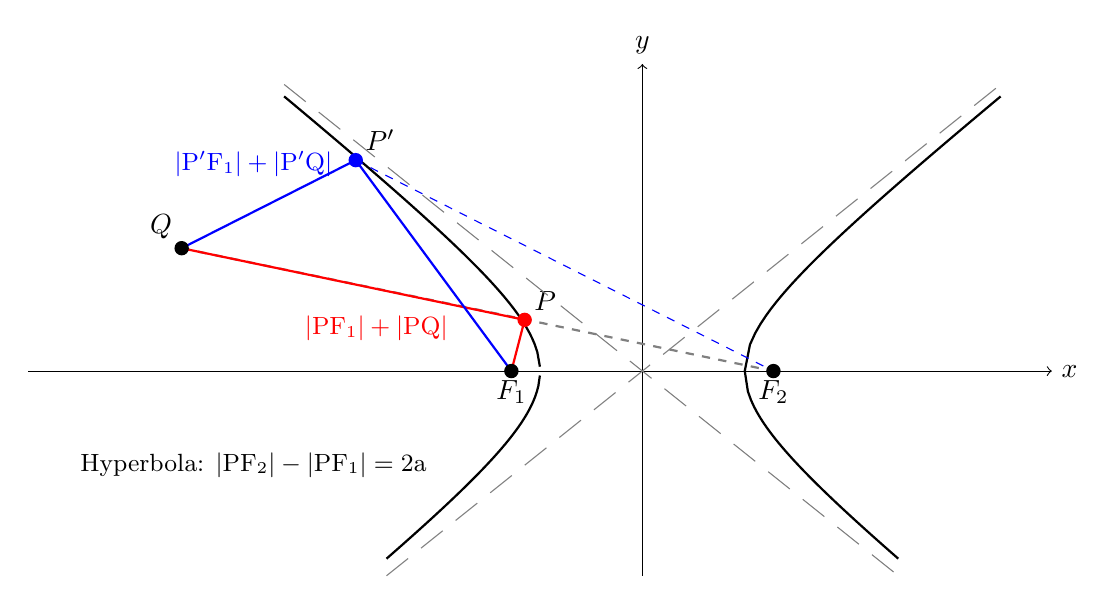
\begin{tikzpicture}[scale=1.3]
    % 坐标轴
    \draw[->] (-6,0) -- (4,0) node[right] {$x$};
    \draw[->] (0,-2) -- (0,3) node[above] {$y$};
    
    % 双曲线参数: a=1, b=0.8, c=1.28
    % 左支
    \draw[thick, black] plot[domain=-3.5:-1, samples=100] 
        (\x, {0.8*sqrt(\x*\x - 1)});
    \draw[thick, black] plot[domain=-2.5:-1, samples=100] 
        (\x, {-0.8*sqrt(\x*\x - 1)});
    % 右支
    \draw[thick, black] plot[domain=1:3.5, samples=50] 
        (\x, {0.8*sqrt(\x*\x - 1)});
    \draw[thick, black] plot[domain=1:2.5, samples=50] 
        (\x, {-0.8*sqrt(\x*\x - 1)});
    
    % 焦点
    \node[below] at (-1.28,0) {$F_1$};
    \node[below] at (1.28,0) {$F_2$};
    
    % Q点
    \coordinate (Q) at (-4.5, 1.2);
    \node[above left] at (Q) {$Q$};
    
    % P点(精确交点,已计算得 x ≈ -1.15, y ≈ 0.295)
    \coordinate (P) at (-1.15, 0.50);
    \node[above right] at (P) {$P$};
    
    % P'点(另一个左支点,x = -2.8, y = 0.8*sqrt(2.8^2-1) ≈ 2.06)
    \coordinate (Pprime) at (-2.8, 2.06);
    \node[above right] at (Pprime) {$P'$};
    
    % Q-F2连线 (蓝色虚线)
    \draw[gray, thick, dashed] (Q) -- (1.28,0);
    
    % 实际光线: F1 -> P (红色实线)
    \draw[red, thick] (-1.28,0) -- (P);
    % 实际光线: P -> Q (红色实线)
    \draw[red, thick] (P) -- (Q);
    
    % 假想光线: F1 -> P' (灰色虚线)
    \draw[blue, thick] (-1.28,0) -- (Pprime);
    % 假想光线: P' -> Q (灰色虚线)
    \draw[blue, thick] (Pprime) -- (Q);
    % 辅助线: P' -> F2 (灰色细虚线)
    \draw[blue, thin, dashed] (Pprime) -- (1.28,0);
    
    \fill[black] (-1.28,0) circle (2pt);
    \fill[black] (1.28,0) circle (2pt);
    \fill[black] (Q) circle (2pt);
    \fill[red] (P) circle (2pt);
    \fill[blue] (Pprime) circle (2pt);
%   % 顶点
%   \fill[black] (-1,0) circle (1pt);
%   \fill[black] (1,0) circle (1pt);
%   \node[below] at (-1,0) {$-a$};
%   \node[below] at (1,0) {$a$};
    
    % 光程标注
    \node[red, above] at (-2.6, 0.2) {\small $|\rm PF_1|+|\rm PQ|$};
    \node[blue, above] at (-3.8, 1.8) {\small $|\rm P'F_1|+|\rm P'Q|$};

    % 渐近线
    % 渐近线的斜率为 b/a = 0.8
    % y = 0.8x 和 y = -0.8x
    \draw[gray, thin, dash pattern=on 10pt off 6pt] (-2.5, {-0.8*2.5}) -- (3.5, {0.8*3.5});
    \draw[gray, thin, dash pattern=on 10pt off 6pt] (-3.5, {0.8*3.5}) -- (2.5, {-0.8*2.5});

    \node[black, below] at (-3.8, -0.7) {\small Hyperbola: $|\rm PF_2|-|\rm PF_1|=2a$};
\end{tikzpicture}